\documentclass{acm_proc_article-sp}
\usepackage{graphicx}
\usepackage{epstopdf}
\usepackage{subfigure}
\usepackage{multirow}
% algorithm package
\usepackage{algorithm}
\usepackage{algorithmic}
\usepackage{indentfirst}
\renewcommand{\algorithmicrequire}{ \textbf{Initialization:}}
\renewcommand{\algorithmicensure}{ \textbf{Recurrence:}}

\begin{document}

\title{Datapath Synthesis for Overclocking: Online Arithmetic for Latency-Accuracy Trade-offs}


\numberofauthors{1} %  in this sample file, there are a *total*
% of EIGHT authors. SIX appear on the 'first-page' (for formatting
% reasons) and the remaining two appear in the \additionalauthors section.
%
\author{
% 1st. author
\alignauthor
Authors
%Kan Shi, David Boland and George A. Constantinides\\
%       \affaddr{Department of Electrical and Electronic Engineering}\\
%       \affaddr{Imperial College London}\\
%       \affaddr{London, UK}\\
%       \email{\{k.shi11, david.boland03, g.constantinides\}@imperial.ac.uk}
%\and  % use '\and for second row
}

\maketitle

\begin{abstract}
In this paper we take a fresh look at Online Arithmetic, originally proposed for digit-serial operation, and synthesize unrolled digit-parallel online operators to allow for graceful degradation under overclocking. We quantify the impact of timing violation on key arithmetic primitives, and show that substantial performance benefits can be obtained in comparison to binary arithmetic. Since timing errors are generated in least significant digits with online arithmetic, less impact is caused than conventional implementations. Using analytical models and empirical FPGA results, we demonstrate an error reduction over $89\%$ and an improvement in SNR of over 20dB for the same clock rate.
%Digital circuits are currently designed to ensure timing closure. Releasing this constraint by allowing timing violations could lead to significant performance improvements, but conventional forms of computer arithmetic do not fail gracefully when pushed beyond deterministic operation. In this paper we take a fresh look at Online Arithmetic, originally proposed for digit serial operation, and synthesize unrolled digit parallel online operators to allow for graceful degradation. We quantify the impact of timing violation on key arithmetic primitives, and show that substantial performance benefits can be obtained in comparison to binary arithmetic. Since timing errors are caused by long carry chains, these result in errors in least significant digits with online arithmetic, causing less impact than conventional implementations. Using analytical models and empirical FPGA results from an image processing application, we demonstrate an error reduction over 89\% and an improvement in SNR of over 20dB for the same clock rate.
\end{abstract}
%
%\vspace{-1.3ex}
% A category with the (minimum) three required fields
%\category{H.4}{Information Systems Applications}{Miscellaneous}
\category{B.2.4}{Arithmetic and Logic Structures}{High-Speed Arithmetic}[Algorithms,Cost/performance]

%\category{D.2.8}{Software Engineering}{Metrics}[complexity measures, performance measures]
\vspace{-1ex}
\terms{Design, Performance, Reliability}
\vspace{-1ex}
\keywords{Online Arithmetic, Overclocking, Imprecise Design} % NOT required for Proceedings
%\vspace{-.5ex}

\section{Introduction}
<<<<<<< HEAD

Circuit performance has increased tremendously over the past decades with the continuous scaling of CMOS technology such that they occupy less area and operate faster. Typically static-timing analysis incorporates safety margins for timing closure. However, continuing with this approach could become very expensive in the short term future. As circuit dimensions scale down, it is increasingly difficult to maintain low relative manufacturing-variation. Because timing margins in static-analysis tools increase with process variability, designing for worst-case delay in circuits becomes increasingly costly as relative process variation increases.\vspace{-1.2ex}
=======
Circuit performance has increased tremendously over the past decades with the continuous scaling of CMOS technology such that they occupy less area and operate faster. Typically static-timing analysis incorporates safety margins for timing closure. However, continuing with this approach could become very expensive in the short term future. As circuit dimensions scale down, it is increasingly difficult to maintain low relative manufacturing-variation. Because timing margins in static-analysis tools increase with process variability, designing for worst-case delay in circuits becomes increasingly costly as relative process variation increases.\vspace{-1ex}
>>>>>>> kan

While datapath can be pipelined to increase clock frequency, this does not reduce overall computational latency. In  embedded applications, which often have strict latency requirements, or in any datapath containing feedback, where C-slow retiming is inappropriate, pipelining does not help meet performance targets. To overcome these problems, a large volume of studies have demonstrated that relaxing the absolute datapath-accuracy requirements can provide the freedom to create designs with better performance or energy efficiency \cite{Razor2004,Gupta2013TransCADICS,NonUniformScaling,Undersigned2x2multiplier}.\vspace{-1ex}
%Our previous work also demonstrated that allowing timing violations to happen would be of benefit in many applications, because the worst case only happens with a very small probability.

<<<<<<< HEAD
Most research in this area focuses on standard binary arithmetic \cite{Gupta2013TransCADICS,NonUniformScaling}, which potentially suffers from large magnitude of timing errors. This is because, in standard arithmetic operators such as ripple-carry adders, the most significant digit (MSD) is updated \emph{last} due to carry propagation, so timing violation initially affects the MSD of the result. In this paper, for the first time we attempt to solve this problem by adopting an alternative form of MSD-first arithmetic known as online arithmetic. We evaluate the probabilistic behavior of basic arithmetic primitives with different types of arithmetic when operating beyond the deterministic clocking region. We suggest that in comparison to conventional arithmetic, operators employing this arithmetic are less sensitive to overclocking, because timing errors only affect the least significant digits. To support this hypothesis, we propose probabilistic models of error for an online multiplier. We back up the models with experimental results on an image processing application. We demonstrate that our novel design methodology can lead to substantial performance benefits compared to the design method using conventional arithmetic. The contributions of this paper are:\vspace{-1ex}

=======
However, we notice that most research in this area focuses on standard binary arithmetic \cite{Gupta2013TransCADICS,NonUniformScaling,Undersigned2x2multiplier}, which potentially suffers from large magnitude of timing errors. This is because, in standard arithmetic operators such as ripple-carry adders, the most significant digit (MSD) is updated \emph{last} due to carry propagation, so timing violation initially affects the MSD of the result. In this paper, for the first time we attempt to solve this problem by adopting an alternative form of MSD-first arithmetic known as online arithmetic. We evaluate the probabilistic behavior of basic arithmetic primitives with different types of arithmetic when operating beyond the deterministic clocking region. We suggest that in comparison to conventional arithmetic, operators employing this arithmetic are less sensitive to overclocking, because timing errors only affect the least significant digits. To support this hypothesis, we propose probabilistic models of error for an online multiplier. We back up the models with experimental results on an image processing application. We demonstrate that our novel design methodology can lead to substantial performance benefits compared to the design method using conventional arithmetic. A summary of the main contributions of this paper are as follows:
>>>>>>> kan
%
\begin{itemize}
\vspace{-2ex}
  \item to our knowledge, the first ``overclocking friendly'' computer arithmetic,\vspace{-.7ex}
  \item probabilistic models of overclocking errors for a digit-parallel online multiplier,\vspace{-.7ex}
  \item analytical and empirical results which demonstrate that the impact of timing violations is ameliorated with online arithmetic and that large performance benefits can be achieved.\vspace{-.7ex}
\end{itemize}



%For instance, the Razor project was proposed to shave the conservative timing margins by overscaling the supply voltage while monitoring the output error rates. It has demonstrated that over $30\%$ energy efficiency can be obtained by allowing $1\%$ output errors. Lu et al. proposed a simplified datapath to speculate the original logic functions for performance benefits. Palem et al. described a voltage scaling technique that employs different voltage regions for different bits along a carry chain in a ripple carry adder. Kulkarni et al. developed an underdesigned multiplier unit, of which the the worst case was replaced by a normal case based on the straight-forward Karnaugh-Map analysis. In addition, our previous work has demonstrated that

% Meanwhile, drastic variations have been introduced by higher integration densities and progressively stringent requirements have been placed on circuit performance. In order to ensure an absolutely correct functionality across various operating conditions, hardware designers tend to employ very conservative safety margins for timing closure.

%In order to meet the stringent latency requirement, a large volume of current studies has demonstrated that, FPGA-based accelerators can be employed to achieve significant performance gains over software designs across a wide range of applications. However, one of the major obstacles of these accelerators is that they typically operate at much lower clock frequencies in comparison to general purpose processors (GPPs) or graphics processing units (GPUs). While the standard approaches such as heavily pipeline the datapath can be used to boost the frequency, the overall latency will not be reduced. Besides, the conservative safety margin will not be removed by these approaches.







\section{Background}
\subsection{Online Arithmetic}
In conventional arithmetic, the computation results are generated either from the least significant digit (LSD), e.g. addition and multiplication, or the MSD, e.g. division and square root. This inconsistency the direction of data-flow can result in large latencies when propagating data among different operations. To tackle this problem, online arithmetic has been proposed and studied over the past few decades \cite{Ercegovac_OnlineOverview,Ercegovac_OnlineMult,Online_Trunc}. Both the inputs and outputs are processed in a MSD-first manner using online arithmetic, enabling parallelism among multiple operations. Therefore the overall latency can be greatly reduced.
\vspace{-1ex}
%Another advantage of online arithmetic is that computations can be dynamically terminated based on the required precision [xxx]. For instance, traditionally $2N$ digits of results will be generated in a $N$-digit multiplier, while only the most significant $N$ digits will be used for successive computations while the $N$ LSDs will be discarded. In contrast, the computation latency can be saved using online arithmetic, which can be finished immediately if the first $N$ digits of results are obtained.

Originally online arithmetic was designed for digit-serial operation. In order to generate the first output digit, $\delta$ digits of inputs are required, as illustrated in Figure \ref{Fig:OnlineDataFlow}. $\delta$ is known as the online delay, which is a constant, independent of the precision in a given operation. For ease of discussion, the input to our circuit is normalized to a fixed point number in the range $(-1,1)$. Based on this premise, the online representations of $N$-digit operands and result at iteration $j$ are given by (\ref{Eq:Online_Operands}) for $j\in[-\delta,N-1]$ and $r$ denotes the radix \cite{Ercegovac_Book}.
\vspace{-1ex}
%
\begin{figure}[htbp]
  \centering
  \vspace{-2.5ex}
  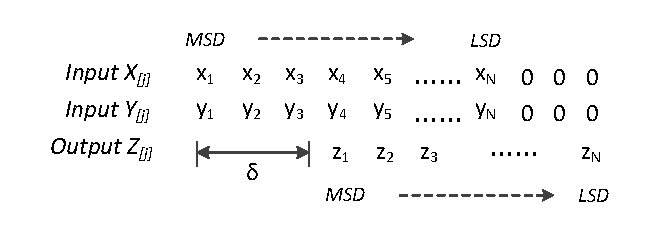
\includegraphics[width=.44\textwidth]{./Figures/OnlineArithmetic_DataFlow.pdf}
  \vspace{-3ex}
  \caption{Dataflow in digit-serial Online Arithmetic.}
  %\vspace{-1.5ex}
  \label{Fig:OnlineDataFlow}
\end{figure}
%
\begin{eqnarray}\label{Eq:Online_Operands}
\footnotesize
  X_{[j]}=\sum_{i=1}^{j+\delta}x_ir^{-i},~Y_{[j]}=\sum_{i=1}^{j+\delta}y_ir^{-i},~Z_{[j]}=\sum_{i=1}^{j}z_ir^{-i}
\normalsize
\end{eqnarray}
%
<<<<<<< HEAD
MSD-first operation in online arithmetic operations is possible because they adopt a redundant number system \cite{RedundantNumber}, in which each digit is represented with a redundant digit set $\{-a, \cdots,\\-1, 0, 1, \cdots, a\}$, where $a\in[r/2,r-1]$. Due to the redundancy, the MSDs of the result can be estimated only based on partial information of the inputs and then the value of the number can be revised by the following digits.

\subsection{Radix-2 Digit-parallel Online Adder \label{OnlineAdderSection}}
Adders serve as a critical building block for arithmetic operations. To perform digit-parallel online addition, a redundant adder can be directly utilized. The adder structure diagram is shown in Figure~\ref{Fig:Radix2SD_adder}. A major advantage with the redundant number system over the standard ripple-carry based arithmetic is that the propagation of carry is eliminated, resulting in a precision-independent computation time for addition. As seen in Figure~\ref{Fig:Radix2SD_adder}, the computation delay of this adder is only 2 full adder (FA) delays for any operand word-length, with the cost of one extra FA for each digit of operands. This makes online adder structures suitable for building up more complex arithmetic operators such as multipliers \cite{RedundantMult_1987,RedundantMult_1985}.
=======
MSD-first operation in online arithmetic is possible because they adopt a redundant number system \cite{RedundantNumber}, in which each digit is represented with a redundant digit set $\{-a, \cdots,-1,\\0, 1, \cdots, a\}$, where $a\in[r/2,r-1]$. Due to the redundancy, the MSDs of the result can be estimated only based on partial information of the inputs and then the value of the number can be revised by the following digits.

\subsection{Radix-2 Digit-parallel Online Adder}\label{subsec:OnlineAdder}
Adders serve as a critical building block for arithmetic operations. To perform digit-parallel online addition, a redundant adder can be directly utilized. The adder structure diagram is shown in Figure~\ref{Fig:Radix2SD_adder}. A major advantage with the redundant number system over the standard ripple-carry based arithmetic is that the propagation of carry is eliminated, resulting in a precision-independent computation time for addition. As seen in Figure~\ref{Fig:Radix2SD_adder}, the computation delay of this adder is only 2 full adder (FA) delays for any operand word-length, with the cost of one extra FA for each digit of operands. This makes online adder suitable for building up more complex arithmetic operators such as multipliers to accelerate the sum of partial products \cite{RedundantMult_1987,RedundantMult_1985}.
% 
% Therefore it is unlikely that timing violations happen on the online adder. For this reason, this adder structure has been widely used as a part of other arithmetic operators such as multipliers to accelerate the sum of partial products
>>>>>>> kan
%
\begin{figure}
%\centering
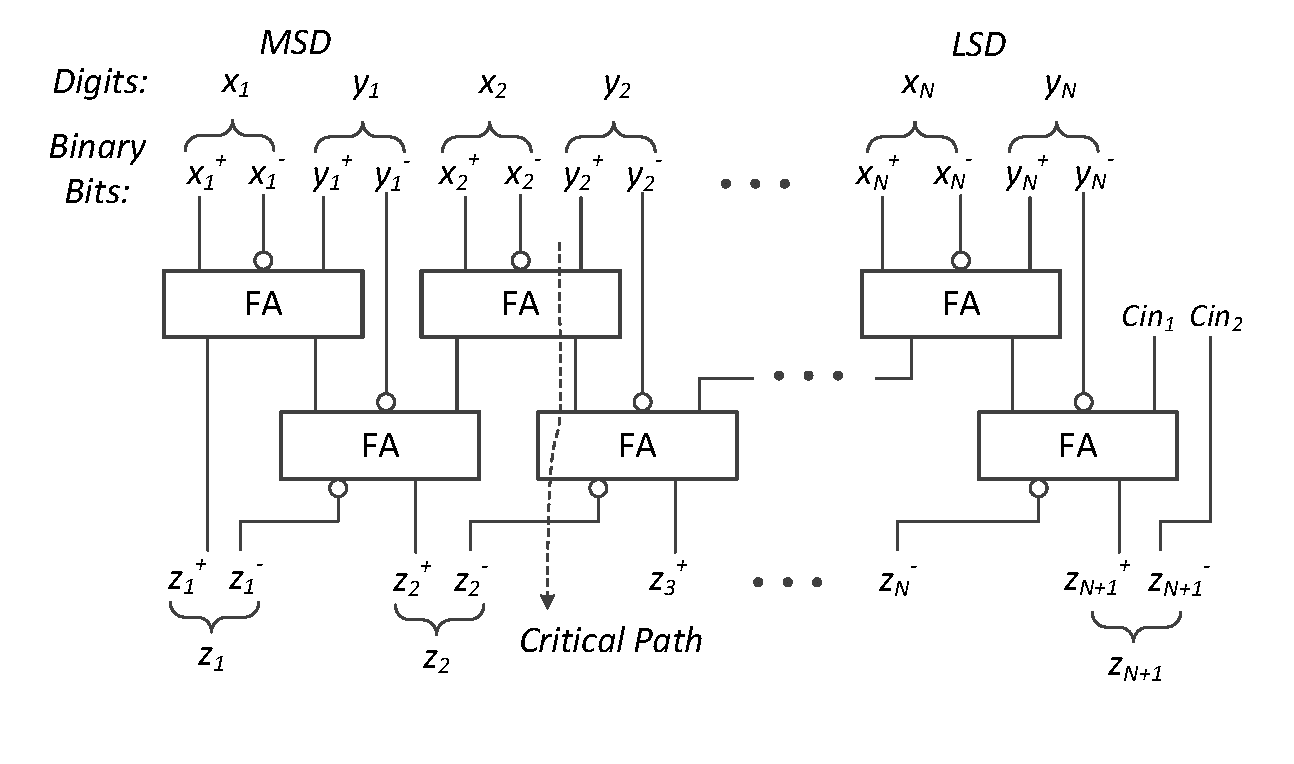
\includegraphics[width=.5\textwidth]{./Figures/SDAdder.pdf}
\vspace{-8.5ex}
\caption{An $N$-digit radix-2 unrolled online adder.}
\label{Fig:Radix2SD_adder}
\end{figure}

%\section{Online Multiplier}
<<<<<<< HEAD
\subsection{Radix-2 Digit-parallel Online Multiplierw \label{OnlineMultSection}}
%\vspace{-1ex}
Multiplication is another key primitive of arithmetic operations. Typically the online multiplication is performed in a recursive digit-serial manner, as illustrated in Algorithm~\ref{Algorithm:OnlineMult} where both inputs and outputs are $N$-digit number as represented in~(\ref{Eq:Online_Operands}). For a given iteration $j$, the product digit $z_j$ is generated through a selection function $sel()$. From the radix (r) and a chosen digit set, there always exists an appropriate selection method and a value of $\delta$ which ensure convergence. As radix-2 is used most commonly in computer arithmetic, we keep $r=2$ throughout this paper with the corresponding redundant digit set $\{\overline{1},0,1\}$. In this case we have $\delta=3$, and $sel()$ is given by (\ref{Eq:SelFunc_OM}) \cite{Oregon_OnlineNetwork}. It can be seen that the decision is made only based on 1 integer bit and 1 fractional bit of $W_{[j]}$.
=======
\subsection{Radix-2 Digit-parallel Online Multiplier}\label{subsec:OnlineMultiplier}
%\vspace{-1ex}
Multiplication is another key primitive of arithmetic operations. Typically the online multiplication is performed in a recursive digit-serial manner, as illustrated in Algorithm~\ref{Algorithm:OnlineMult} where both inputs and outputs are $N$-digit number as represented in~(\ref{Eq:Online_Operands}). For a given iteration $j$, the product digit $z_j$ is generated through a selection function $sel()$. For the radix $r$ and a chosen digit set, there exits an appropriate selection method and a value of $\delta$ which ensure convergence. As radix-2 is used most commonly in computer arithmetic, we keep $r=2$ throughout this paper with the corresponding redundant digit set $\{\overline{1},0,1\}$. In this case we have $\delta=3$, and $sel()$ is given by (\ref{Eq:SelFunc_OM}) \cite{Oregon_OnlineNetwork}, from which it can be seen that the decision is made only based on 1 integer bit and 1 fractional bit of $W_{[j]}$.
%In order to ensure the convergence of the algorithm, appropriate selection method and the value of $\delta$ should be determined on the basis of radix $r$ and the digit set
>>>>>>> kan

\begin{algorithm}[tbp]
  \caption{Online Multiplication}
  \begin{algorithmic}[1]
    \REQUIRE~$X_{[-\delta]}=Y_{[-\delta]}=P_{[-\delta]}=0$
    \ENSURE~$for~~ j=-\delta,~-\delta+1,~\cdots,~N-1 ~~do$
      \begin{eqnarray}\label{Eq:OnlineMult_General}
        \begin{matrix}
          H_{[j]}   & = & r^{-\delta}\left(x_{j+\delta+1}\cdot Y_{[j+1]}+y_{j+\delta+1}\cdot X_{[j]}\right)\\
          W_{[j]}   & = & P_{[j]} + H_{[j]}\\
          z_j       & = & sel(W_{[j]})\\
          P_{[j+1]} & = & r\left(W_{[j]}-z_j\right)
        \end{matrix}
      \end{eqnarray}
  \label{Algorithm:OnlineMult}
  \vspace{-2ex}
  \end{algorithmic}
\end{algorithm}
\vspace{-2ex}

\vspace{-2ex}
\begin{eqnarray}\label{Eq:SelFunc_OM}
\small
  sel(W_{[j]})=\begin{cases}
    1 & \text{ if } W_{[j]} \geqslant \frac{1}{2} \\
    0 & \text{ if } -\frac{1}{2}\leqslant W_{[j]}<\frac{1}{2} \\
    \overline{1} & \text{ if } W_{[j]}<-\frac{1}{2}
  \end{cases}
\normalsize
\end{eqnarray}
%\vspace{-2ex}

Algorithm \ref{Algorithm:OnlineMult} can be synthesized into a unrolled digit parallel structure as shown in  Figure~\ref{Fig:Radix2OnlineMultiplier}(a). In an $N$-digit OM, there are totally $N+\delta$ stages, of which the online inputs are generated from the appending logic according to (\ref{Eq:Online_Operands}). For each stage, an online adder is used as shown in Figure~\ref{Fig:Radix2OnlineMultiplier}(b). The SDVM module performs the signed-digit vector multiplication. When $r=2$ and the digit set $\{\overline{1},0,1\}$ is used, the implementation of SDVM is straight forward, because for instance the output of $(y_{j+\delta+1}\cdot X_{[j]})$ is 0, $X_{[j]}$ or $-X_{[j]}$ when $y$ is equal to $0$, $1$ and $-1$ respectively.\vspace{-1ex}

\begin{figure}[tbp]
\centering
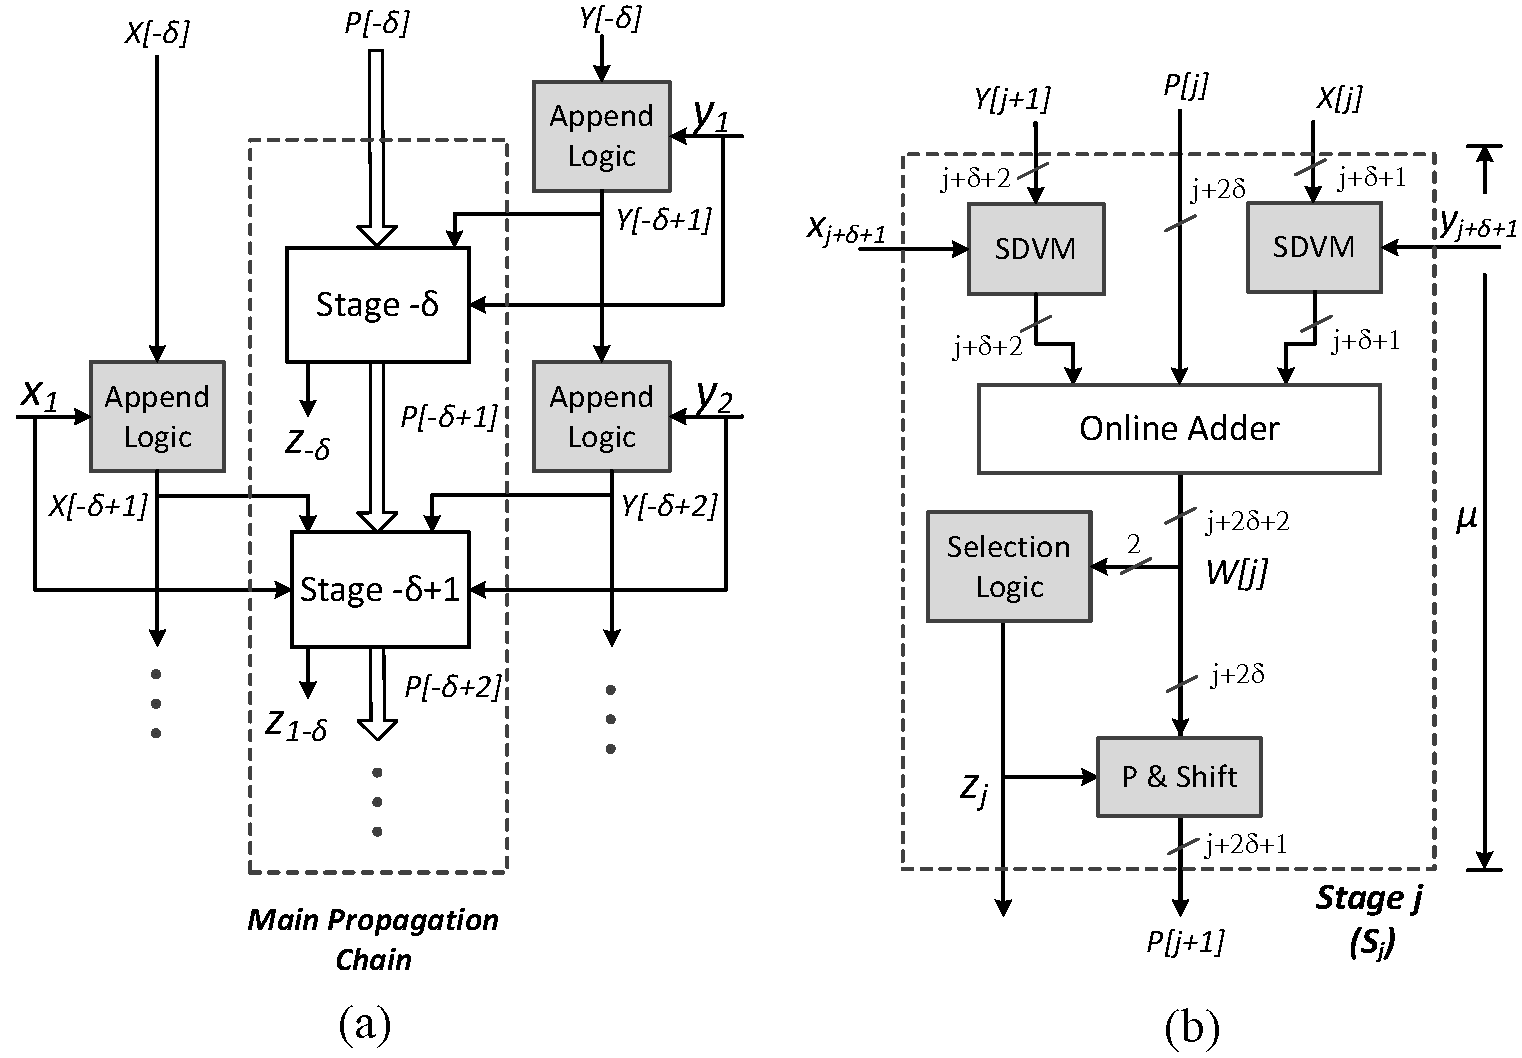
\includegraphics[width=.49\textwidth]{./Figures/OnlineMult_Unrolled.pdf}
\vspace{-4ex}
\caption{(a) Synthesis of Algorithm 1 into a digit-parallel online multiplier (b) Structure of one stage, in which the maximum digit widths of signals are labeled.}
\vspace{-2ex}
\label{Fig:Radix2OnlineMultiplier}
\end{figure}

Instead of duplicating the digit-serial implementation $N+\delta$ times, each stage in the digit-parallel architecture can be optimized for area reduction. For instance, the SDVM modules and the appending logic are not required in the last $\delta$ stages because the inputs are 0. This leads to a smaller online adder in these stages. Similarly for the first $\delta$ stages the selection logic can be removed, as the first digit of the result is generated at stage 0 ($S_0$).

%\section{Analysis of The Critical Path}
%
%Suppose a chain is generated at the first stage $S_{-\delta}$ and is propagated to the final stage $S_{N-1}$. This corresponds to $d(\tau)=N+\delta$ and hence the critical path delay of the OM is then given by (\ref{Eq:WorstCaseDelay_NaiveAnalysis}). Note that this value is normally employed by the timing analysis tools together with a guard-band to ensure a correct functionality across a variety of operating conditions.
%
%\begin{eqnarray}\label{Eq:WorstCaseDelay_NaiveAnalysis}
%  \mu_{OM\_structural} = (N+\delta)\cdot \mu
%\end{eqnarray}
%%
%For a given stage $S_\tau$ when inputs are initially introduced, we have $W_{[\tau]}=H_{[\tau]}$ as $P_{[\tau]}=0$. From (\ref{Eq:OnlineMult_General}) the maximum word-length of $H_{[\tau]}$ and $P_{[\tau]}$ is $(\tau+2\delta+2)$ and $(\tau+2\delta)$, respectively. Thus the propagation of $P_{[\tau]}$ will only affect the first $(\tau+2\delta)$ MSDs of $W_{[\tau]}$. As an example, the maximum word-length of $P_{[-2]}$ is 4 digits while the value of $H_{[-2]}$ is 6. After delay $\mu$ from the start of computation, only the first 4 digits of $W_{[-2]}$ will be changed by the propagation of $P_{[-2]}$, as labeled on the segment of $P_{[-2]}$ in Figure~\ref{Fig:TimingGraph_OM}. During each propagation, this value is reduced by 1 due to the shifting to derive $P_{[j+1]}$ in (\ref{Eq:OnlineMult_General}). Finally this chain annihilates if the number shrinks to 1, because for all possible changes as listed in Table~\ref{Tab:Annihilation}, the propagation output keeps unchanged. In the previous example, the chain generated at $S_{-3}$ will annihilate at $S_1$ as shown in Figure \ref{Fig:TimingGraph_OM}. Besides, chains generated at other stages with the maximum lengths are also depicted for a 3-digit OM. It can be seen that the actual worst-case delay is $5\mu$, instead of $6\mu$ as predicted by (\ref{Eq:WorstCaseDelay_NaiveAnalysis}).
%%
%\begin{figure}[tbp]
%\centering
%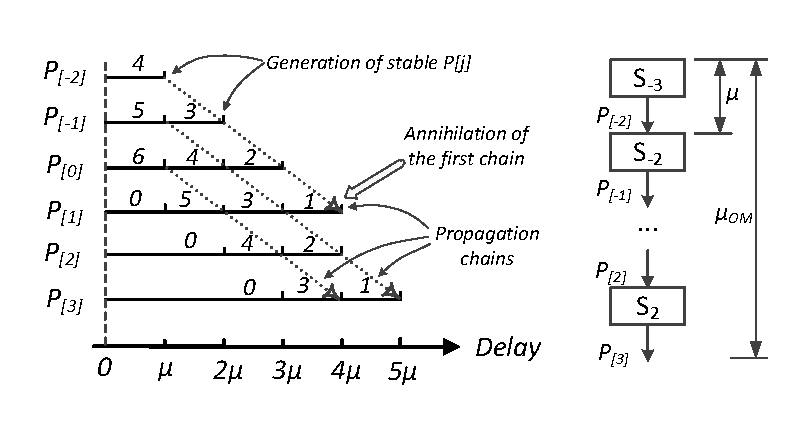
\includegraphics[width=.5\textwidth]{./Figures/Timing_3DigitOM.pdf}
%\vspace{-5ex}
%\caption{All possible chains with the maximum length in a 3-digit online multiplier. The numbers on the line segment represent the number of the updated MSDs of $W_{[j]}$.}
%\label{Fig:TimingGraph_OM}
%\end{figure}
%%
%\begin{table}[tbp]
%\centering
%\caption{All the combinations of ${W}_{[j]}$ of which 2 MSBs might change. Together with the corresponding $z_j$ and the integer bit of $P_{[j+1]}$.}
%\begin{tabular}{|c|c|c|c|}
%\hline
%${W}_{[j]}$&$z_j$&$P_{[j+1]}=2(W_{[j]}-z_j)$\\ \hline
% $0.0\rightarrow1.0$ & $0\rightarrow\overline{1}$ & $0\rightarrow0$\\ \hline
% $0.1\rightarrow1.1$ & $1\rightarrow0$ & $1\rightarrow1$\\ \hline
% $1.0\rightarrow0.0$ & $\overline{1}\rightarrow0$ & $0\rightarrow0$\\ \hline
% $1.1\rightarrow0.1$ & $0\rightarrow{1}$ & $1\rightarrow1$\\  \hline
%\end{tabular}
%\label{Tab:Annihilation}
%\vspace{-2ex}
%\end{table}
%
%In general for a given value of $\tau$, the maximum value of $d(\tau)$ is bounded by two constraints. On one hand, the chain length cannot be greater than $N-1$. On the other hand, the altered digit number of $P_{[\tau+1]}$ will eventually reduced to 1. The combination of both gives (\ref{Eq:Bound_ChainLength}).
%%
%\begin{eqnarray}\label{Eq:Bound_ChainLength}
%  d(\tau)_{max}=Min(N-1-\tau,~\tau+2\delta+1)
%\end{eqnarray}
%For all values of $\tau$ in (\ref{Eq:Bound_GenChain}), the critical path delay of the OM is then given by (\ref{Eq:MaxChainLength_OneStage}).
%%
%\begin{eqnarray}\label{Eq:MaxChainLength_OneStage}
%  \mu_{OM}=Max(d(\tau)_{max})\cdot\mu
%\end{eqnarray}
%%
%Substituting (\ref{Eq:Bound_GenChain}) and (\ref{Eq:Bound_ChainLength}) into (\ref{Eq:MaxChainLength_OneStage}), we obtain the expression of $\mu_{OM}$ in (\ref{Eq:WorstCaseDelay_OM}). The comparison between (\ref{Eq:WorstCaseDelay_NaiveAnalysis}) and (\ref{Eq:WorstCaseDelay_OM}) is illustrated in Figure \ref{Fig:Gap_OM}, from which we see that the OM could run at a higher frequency than predicted from naive structural timing analysis.
%%
%\begin{eqnarray}\label{Eq:WorstCaseDelay_OM}
%  \mu_{OM} = \begin{cases}
%    \frac{N-1}{2}\cdot\mu+4\mu & \text{if N is odd}\\
%    \frac{N-2}{2}\cdot\mu+4\mu & \text{if N is even}
%  \end{cases}
%\end{eqnarray}
%
%%
%\begin{figure}[t]
%    \centering
%    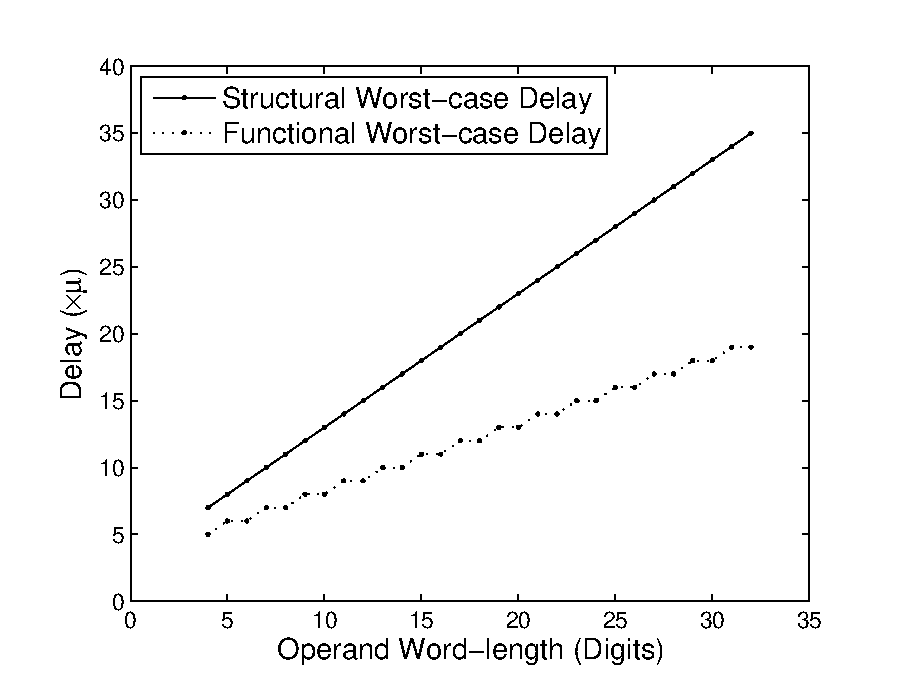
\includegraphics[width=.4\textwidth]{./Figures/Gap.eps}
%    %\vspace{-5ex}
%    \caption{Comparison between the worst-case delay of an online multiplier obtained from (\ref{Eq:WorstCaseDelay_NaiveAnalysis}) and (\ref{Eq:WorstCaseDelay_OM}).}
%\label{Fig:Gap_OM}
%\end{figure}


%\subsection{Probabilistic Model of Overclocking \\Error}
\section{Probabilistic Model of\\Overclocking Error}
As it is unlikely that timing violation happens in the online adder, in this section we model the overclocking error in the radix-2 online multiplier (OM). From Figure~\ref{Fig:Radix2OnlineMultiplier} we observe two types of delay chains. One is caused by generation and propagation of $P_{[j]}$ among different stages. The other is the generation of online inputs $X_{[j]}$ and $Y_{[j]}$ from the appending logic. Since the appending logic is basically wires and simple combinational logic \cite{Online_Conversion}, the overall latency will eventually be determined by the delay of the $P_{[j]}$ path, especially with increasing operand word-lengths. As such, we initially model the delay of each stage within an OM to be a constant value $\mu$, as shown in Figure~\ref{Fig:Radix2OnlineMultiplier}(b). We also assume that the generation of online inputs costs no delay.\vspace{-1ex}

Let $\mu_{OM}$ denote the worst-case delay of an OM. It follows that if the clock period $T_S$ is greater than $\mu_{OM}$, correct results will be sampled. If, however, faster-than-rated sampling frequencies are applied such that $T_S<\mu_{OM}$, timing violations might happen and intermediate results will be sampled, potentially generating errors. For a given $T_S$, the maximum length of error-free propagation is described by (\ref{Eq:MaxChainLength}) where $f_S$ denotes the sampling frequency. To avoid too large frequencies, we always ensure that the first digit of the result will be generated correctly, i.e. $b>\delta$.
%
\begin{eqnarray}\label{Eq:MaxChainLength}
\footnotesize
  b:=\left\lceil \frac{T_S}{\mu} \right\rceil=\left\lceil \frac{1}{\mu\cdot f_S}\right\rceil
  %b:=\left\lceil T_S/{\mu} \right\rceil=\left\lceil {1}/{(\mu\cdot f_S)}\right\rceil
\normalsize
\end{eqnarray}
%
We then model the errors assuming that every digit of each input to our circuit is uniformly and independently generated with the digit set $\{\overline{1},0,1\}$. This assumption will be relaxed in Section \ref{Sec:CaseStudy} where real image data are used.

\subsection{Probability of Timing Violations}
For an $N$-digit OM, let a propagation chain be generated at stage $S_{\tau}$ with the length of $d(\tau)$ digits, then the stage number $\tau$ is bounded by (\ref{Eq:Bound_GenChain}). The presence of timing violation requires $d(\tau)>b$. Besides, the chain cannot propagate over stage $S_{N-1}$. Therefore the bound of parameter $d(\tau)$ is given by (\ref{Eq:Bound_ChainLength}).
%
\begin{eqnarray}\label{Eq:Bound_GenChain}
\tiny
  -\delta\leqslant\tau\leqslant N-1-b=\tau_{max}
\end{eqnarray}
%
\vspace{-5ex}
\begin{eqnarray}\label{Eq:Bound_ChainLength}
  b<d(\tau)\leqslant N-1-\tau
\normalsize
\end{eqnarray}
%
However, the actual length of a propagation chain is dependent upon input patterns. Let $C(\tau)$ represent the specific input pattern of $S_{\tau}$. Generally there are four types of inputs as listed in (\ref{Eq:AllInputCases}). Under the assumption that all digits of input signal are mutually independent, the probability of $C_1\sim C_4$ equal to $1/9$, $4/9$, $2/9$ and $2/9$ respectively.
%
\begin{eqnarray}\label{Eq:AllInputCases}
\footnotesize
  C(\tau)=\left\{\begin{matrix}
    \text{Case 1~(}C_1{):} & x_{\tau+\delta+1}=0,~y_{\tau+\delta+1}=0\\
    \text{Case 2~(}C_2{):} & x_{\tau+\delta+1}\neq0,~y_{\tau+\delta+1}\neq0\\
    \text{Case 3~(}C_3{):} & x_{\tau+\delta+1}\neq0,~y_{\tau+\delta+1}=0\\
    \text{Case 4~(}C_4{):} & x_{\tau+\delta+1}=0,~y_{\tau+\delta+1}\neq0
  \end{matrix}\right.
\normalsize
\end{eqnarray}
%
If all internal signals are reset to 0 initially, then (\ref{Eq:OnlineMult_General}) can be modified to give (\ref{Eq:P_Wordlength}) for $\tau>-\delta$. Consequently no propagation chain will be generated at $S_{\tau}$ if $C(\tau)=C_1$.
%
\begin{eqnarray}\label{Eq:P_Wordlength}
\footnotesize
  \begin{aligned}
    P_{[\tau+1]} &= r\cdot W_{[\tau]}\\
                 &= r^{-\delta+1}(x_{\tau+\delta+1}Y_{[\tau+1]}+y_{\tau+\delta+1}X_{[\tau]})\\
  \end{aligned}
\normalsize
\end{eqnarray}
%
In other cases, a new propagation chain will be generated at $S_{\tau}$. If, for example, the word-length of $P_{[\tau+1]}$ is $D$ digits. That is, $P_{[\tau+1]}$ changes $D$ digits for chain generation. From (\ref{Eq:OnlineMult_General}) we notice that $D=D-1$ when $P_{[\tau+1]}$ propagates to the next stage, because of the 1-digit shifting when computing $P_{[\tau+1]}=r(W_{[\tau]}-z_{\tau})$, and this process is independent of the inputs. Finally this chain is annihilated when $D=1$. Hence the actual chain length corresponds to the word-length of $P_{[\tau+1]}$, of which the value we consider separately for different values of $C(\tau)$.\vspace{-1ex}

According to (\ref{Eq:Online_Operands}) the word-lengths of $X_{[\tau]}$ and $Y_{[\tau+1]}$ are $(\tau+\delta+1)$ digits $(\tau+\delta+2)$ digits, respectively. If $C(\tau)=C_2$, $P_{[\tau+1]}$ embodies the maximum word-length, i.e. $D=\tau+\delta+1+\delta$ from (\ref{Eq:P_Wordlength}). Combining $D$ and (\ref{Eq:Bound_ChainLength}) gives the longest chain length in (\ref{Eq:MaxChainLength_OneStage}).
%
\begin{eqnarray}\label{Eq:MaxChainLength_OneStage}
\footnotesize
  d(\tau)_{max}=Min(D,N-1-\tau)
\normalsize
\end{eqnarray}
%
Since the carry generation, propagation and annihilation behavior from $C_3$ and $C_4$ are identical, we only discuss the situation that $C(\tau)=C_3$. In this case the word-length of $P_{[\tau+1]}$ only depends on that of $Y_{[\tau+1]}$. Besides, we have $Y_{[\tau+1]}=Y_{[\tau]}$ because the appending digit $y_{\tau+\delta+1}=0$. It means $d(\tau)$ becomes dependent of the inputs of previous stage $S_{\tau-1}$. There are 2 possible situations for $\tau>-\delta$ as stated below:
\vspace{-2.5ex}
\begin{itemize}
  \item For the previous stage if $y_{\tau+\delta}\neq0$, then the word-length of $Y_{[\tau]}$ is maximized. Thus $d(\tau)=d(\tau)_{max}-1$.\vspace{-1ex}
  \item If $y_{\tau+\delta}=0$, then $Y_{[\tau]}=Y_{[\tau-1]}$. This is a recursive process and these two judgements will be performed again for $\tau=\tau-1$. It terminates when $\tau=-\delta$ or the first judgement is satisfied.
\end{itemize}
\vspace{-1.5ex}
%
For the first stage where $\tau=-\delta$, (\ref{Eq:P_Wordlength}) can be modified further yielding $P_{[-\delta+1]}=r^{\delta+1}(x_1Y_{[-\delta+1]})$. Therefore the value in (\ref{Eq:MaxChainLength_OneStage}) can only be achieved when $C(-\delta)=C_1$, otherwise $d(-\delta)=0$.\vspace{-1ex}

In summary, we derive Algorithm 2 to go through all possible stages that timing violations may occur and the corresponding inputs. This algorithm returns $Prob(T_S)$, which denotes the probability that timing violations happen in an $N$-digit online multiplier under a given $T_S$. $Prob(i,C(i))$ denotes the probability of the input pattern for stage $i$.
%
\begin{algorithm}[htbp]
  \caption{Probability of Timing Violations}
  \begin{algorithmic}[1]
    \STATE  $Prob(T_S)=0$
    \FORALL {stages $\tau\in\{-\delta,-\delta+1,\cdots,\tau_{upp}\}$ and input cases $C(\tau)\in\{C_1,\cdots,C4\}$}
    \STATE  Determine $d(\tau)$ based on $C(\tau)$
    \IF     {$d(\tau)>b$}
    \STATE  $Prob(T_S)=Prob(T_S)+\prod_{i=-\delta}^{\tau}Prob(i,C(i))$
    \ENDIF
    \ENDFOR
    \RETURN $Prob(T_S)$
  \label{Algorithm:ProbabilityTimingViolation}
  \end{algorithmic}
\end{algorithm}

\subsection{Magnitude of Overclocking Error}
In the presence of timing violation, multiple chains might not be correctly propagated. Let us consider the first chain that timing violation may occur, i.e. $d(\tau)_{max}>b$, denote that it annihilates at $S_{\lambda}$ where $\lambda=\tau+d_{max}(\tau)-1$. Therefore overclocking errors may happen from digit $\lambda$ to digit $N-1$ of the result. In general, the magnitude of overclocking error is given by (\ref{Eq:ErrorMagnitude}), where $z_i$ and ${z_i}'$ denote the correct value and the actual value of the output digit of $S_i$, separately, and $\varepsilon_i\in\{\pm2,\pm1\}$.
%
\begin{eqnarray}\label{Eq:ErrorMagnitude}
\scriptsize
  \left|\varepsilon\right|=\left|\sum_{i=\lambda}^{N-1}2^{-i-1}(z_i-{z_i}')\right|=\left|\sum_{i=\lambda}^{N-1} \varepsilon_i\right|
\normalsize
\end{eqnarray}
%
However, the change of output digits may not result in a different number with online arithmetic, because the number is represented in a redundant form. For instance, the two's complement number $0.111$ can be represented in the online form as $0.10\overline{1}$, $0.1\overline{1}1$ and $0.111$. In contrast, errors will always be generated in this case with conventional arithmetic.


%Specifically as seen in Figure \ref{Fig:TimingGraph_OM}, only the MSD of ${W}_{[\lambda]}$ will change during ${z_\lambda}'\rightarrow z_\lambda$. Therefore $\Delta z_i=z_i-{z_i}'$ could be $\pm1$ according to Table \ref{Tab:Annihilation}. Whereas in other cases, ${W}_{[i]}$ might change 2 MSDs, potentially results in errors being $0$, $\pm1$ and $\pm2$.

%Now we notice that the overclocking error is not a deterministic value for a given $T_S$. Thus instead of directly using (\ref{Eq:ErrorMagnitude}), we employ the expectation of error magnitude across these variations on the condition of the appearance of timing violations as given by (\ref{Eq:Error_Overclocking}) where $\varepsilon_\lambda=\pm2^{-\lambda-1}$ and $\varepsilon_i\in\{0,\pm2^{-i-1},\pm2^{-i}\}$.
%%
%\begin{eqnarray}\label{Eq:Error_Overclocking}
%\scriptsize
%      E(|\varepsilon|)=E\left(\left|\varepsilon_\lambda+\sum_{i=\lambda+1}^{N-1}\varepsilon_i \right|\right)
%\normalsize
%\end{eqnarray}

\subsection{Expectation of Overclocking Error}\label{Sec:MeanError}
For a given $T_S$, the combination of $Prob(T_S)$ and $E(|\varepsilon|)$ in Algorithm 2 and (\ref{Eq:ErrorMagnitude}) yields the overall expectation of overclocking error, as presented in (\ref{Eq:Expectation_Overclocking}). The verification of the proposed model is illustrated in the top row of Figure \ref{Fig:ModelVerification} against the results from Monte-Carlo simulations based on the aforementioned timing model. $T_S$ is normalized with respect to the value from structural timing analysis, i.e. $(N+\delta)\mu$. Note that both results are obtained when assuming the input data are randomly generated following uniform distribution. It can be seen that the modeled value match well with the simulation results. We also verify the models against the FPGA results without timing assumptions, as illustrated in the bottom row in Figure~\ref{Fig:ModelVerification}.
The general behavior of the model is similar to the FPGA implementation, however it does not capture the small increments in errors because we only model the coarse delay which is in units of $\mu$. Whereas the other sources of delay are not modeled, such as the generation of the online inputs and result digits.
%
\begin{eqnarray}\label{Eq:Expectation_Overclocking}
\scriptsize
  E_{ovc}=Prob(T_S)\cdot |\varepsilon|
\normalsize
\end{eqnarray}

\begin{figure}[t]
  \vspace{-2.5ex}
  \centering
  %\vspace{-4ex}
  \subfigure[8-digit]{
  \begin{minipage}{0.24\textwidth}
    %\centering
    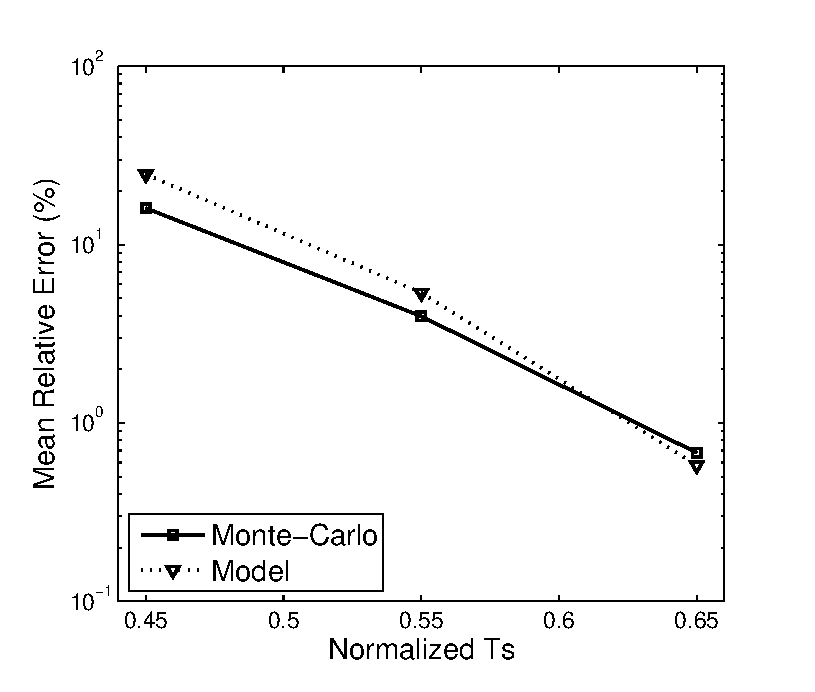
\includegraphics[width=1.7in]{./Figures/WL8_Model.eps}
  \end{minipage}%
  }% This is important! use % to indicate same line, otherwise new line
  \subfigure[12-digit]{
  \begin{minipage}{0.24\textwidth}
    %\centering
    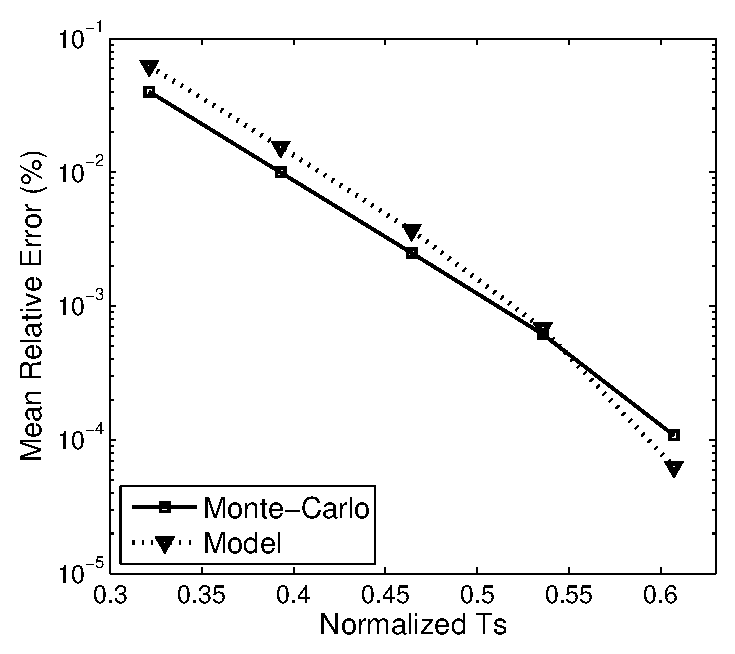
\includegraphics[width=1.7in]{./Figures/WL12_Model.eps}
  \end{minipage}
  }\vspace{-2ex}
  \subfigure[8-digit]{
  \begin{minipage}{0.24\textwidth}
    %\centering
    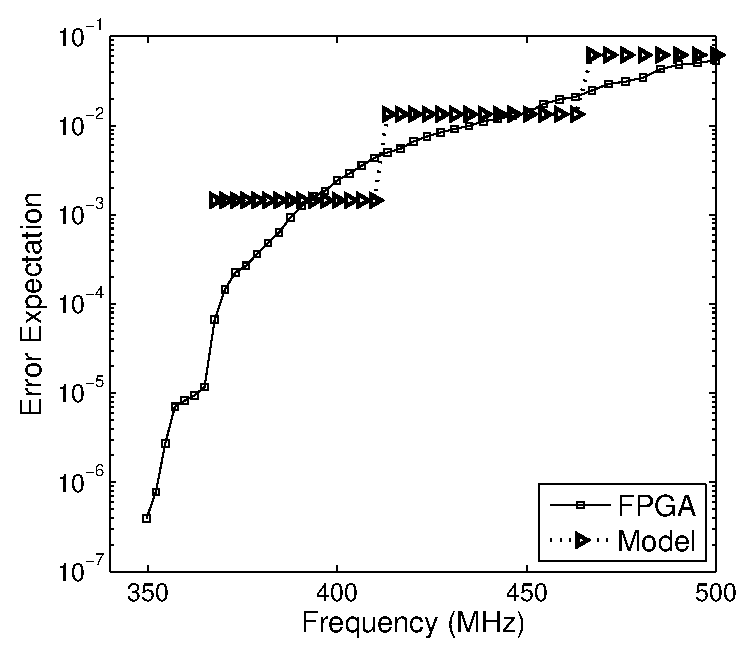
\includegraphics[width=1.7in]{./Figures/Model8.eps}
  \end{minipage}%
  }% This is important! use % to indicate same line, otherwise new line
  \subfigure[12-digit]{
  \begin{minipage}{0.24\textwidth}
    %\centering
    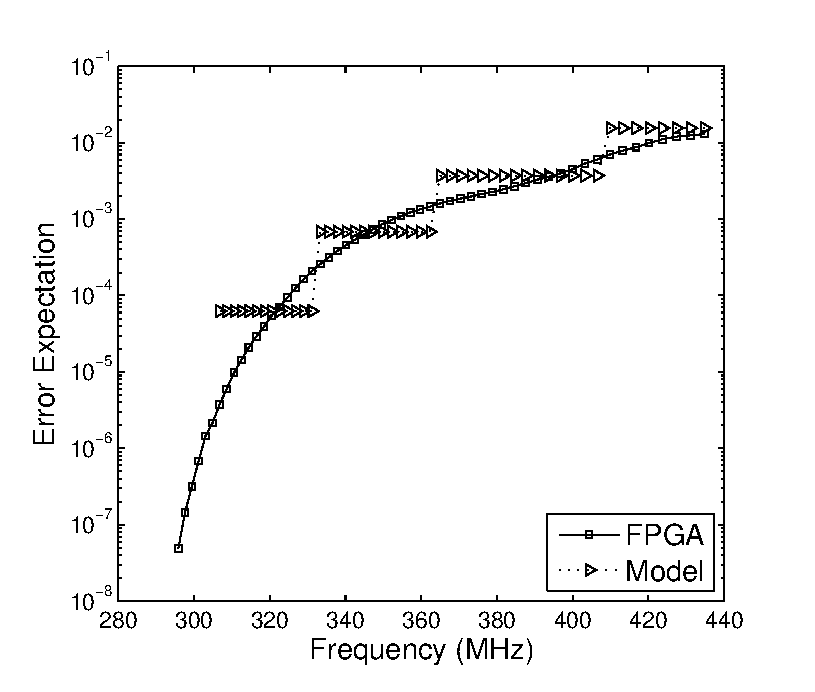
\includegraphics[width=1.7in]{./Figures/Model12.eps}
  \end{minipage}
  }
  \vspace{-2ex}
  \caption{Expectation of overclocking error for online multipliers: verification of the proposed model against Monte-Carlo simulations with timing assumptions (top row) and FPGA results with real timing information (bottom row).}
  \label{Fig:ModelVerification}
  \vspace{-2ex}
\end{figure}

\vspace{-2ex}
For all possible $\tau$ as bounded by (\ref{Eq:Bound_GenChain}), the probability of different chain lengths within an $N$-digit OM and the corresponding magnitude of overclocking error can be obtained, as shown in Figure \ref{Fig:Probability_Error_Mean} with $N=8,12,16,32$, respectively. For a given $T_S$, the overall expectation of overclocking error in (\ref{Eq:Expectation_Overclocking}) can also be computed by (\ref{Eq:PDF_MeanError}).
%
\begin{eqnarray}\label{Eq:PDF_MeanError}
\scriptsize
  E_{ovc}=\sum_{d>b}P_d\cdot\varepsilon_d
\normalsize
\end{eqnarray}
%
From Figure \ref{Fig:Probability_Error_Mean} several observations can be made. First, the error magnitude decreases exponentially with longer chain lengths, because timing violation firstly affects LSDs with online arithmetic. Second, we see that chains with longer delay would happen with greater probabilities in an OM. This is because for the unrolled radix-2 OM, $d(\tau)$ is only dependent upon the inputs for chain generation instead of propagation and annihilation. Thus long chain is generated as long as both input digits are not zeros with the probability of 4/9. Compared to the traditional arithmetic, carry generation, propagation and annihilation are all decided by specific input patterns. This limits the overall probability of long chains. However, we also notice that for chains with long delays, the increasing in likelihood of error is outweighed by the decrease in magnitude of error. Therefore the combination of both results in a decline in error expectation. In contrast, one would expect error expectation to grow faster as the amount of overclocking is increased when using traditional arithmetic because errors occur in MSBs.

%traditional arithmetic, the decrease of probability is offset by the growth of error magnitude, as both of them vary exponentially. Hence the error expectation with respect to each chain delay keeps almost constant. In contrast,

%In addition, carry chains could not be overlapped with traditional arithmetic, whereas long chains might occur simultaneously and mutually overlapped within the OM.
%, because the delay is mainly dependent upon the inputs that generate the chain, while the chain propagation and annihilation will not be affected by the inputs. For the traditional ripple-carry-based arithmetic,
%This finding indicates that the OM is less sensitive to overclocking error than the multiplier using traditional arithmetic, especially when timing violations initially appear.

\begin{figure}[t]
  \vspace{-2.5ex}
  \centering
  \subfigure[8-digit]{
  \begin{minipage}{0.24\textwidth}
    %\centering
    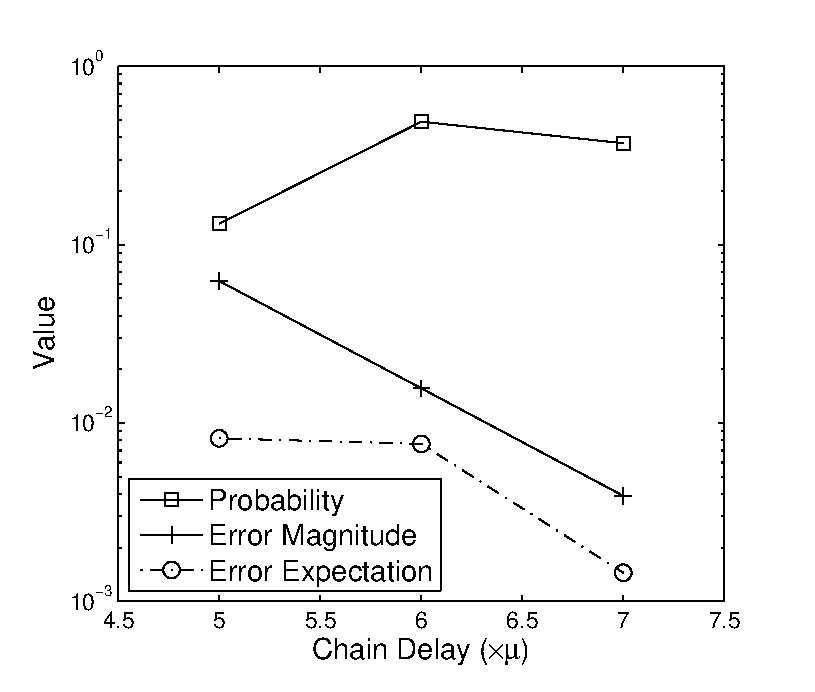
\includegraphics[width=1.7in]{./Figures/PE8.eps}
  \end{minipage}%
  }% This is important! use % to indicate same line, otherwise new line
  \subfigure[12-digit]{
  \begin{minipage}{0.24\textwidth}
    %\centering
    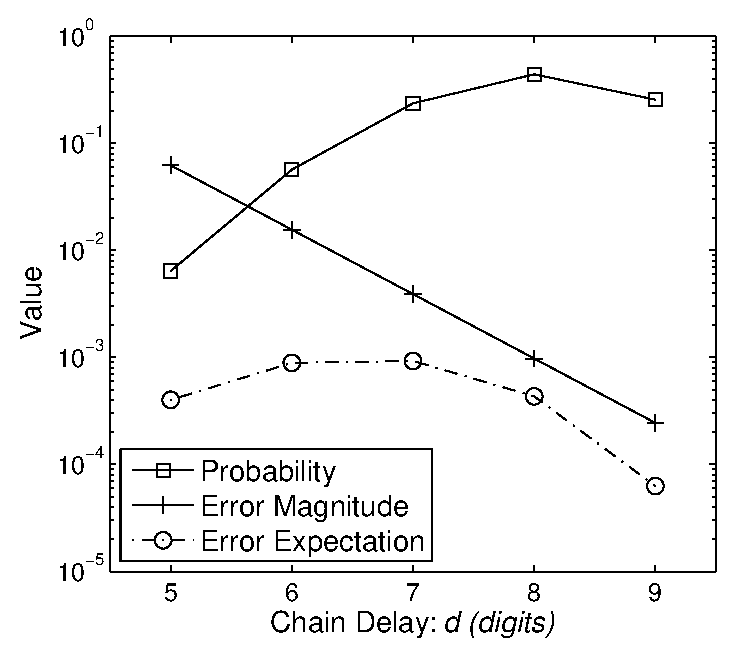
\includegraphics[width=1.7in]{./Figures/PE12.eps}
  \end{minipage}
  }\vspace{-2ex}
  \subfigure[16-digit]{
  \begin{minipage}{0.24\textwidth}
    %\centering
    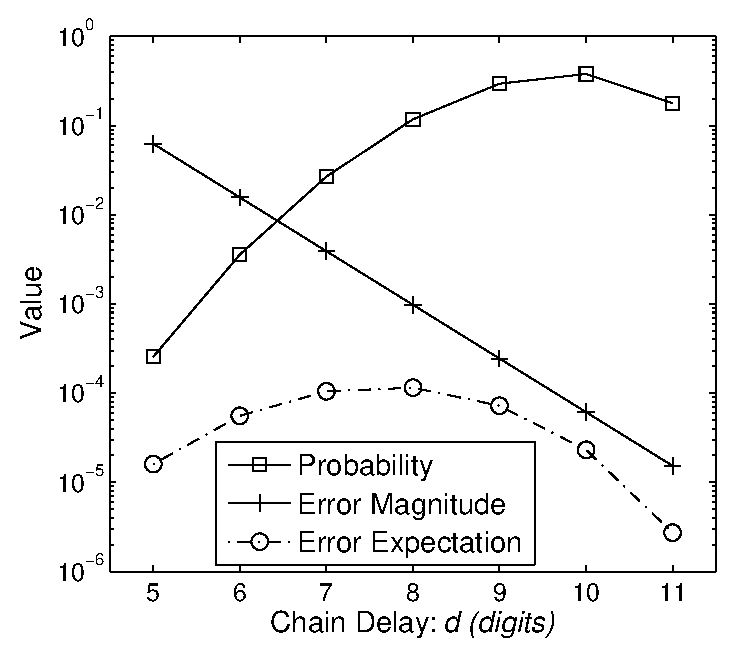
\includegraphics[width=1.7in]{./Figures/PE16.eps}
  \end{minipage}%
  }% This is important! use % to indicate same line, otherwise new line
  \subfigure[32-digit]{
  \begin{minipage}{0.24\textwidth}
    %\centering
    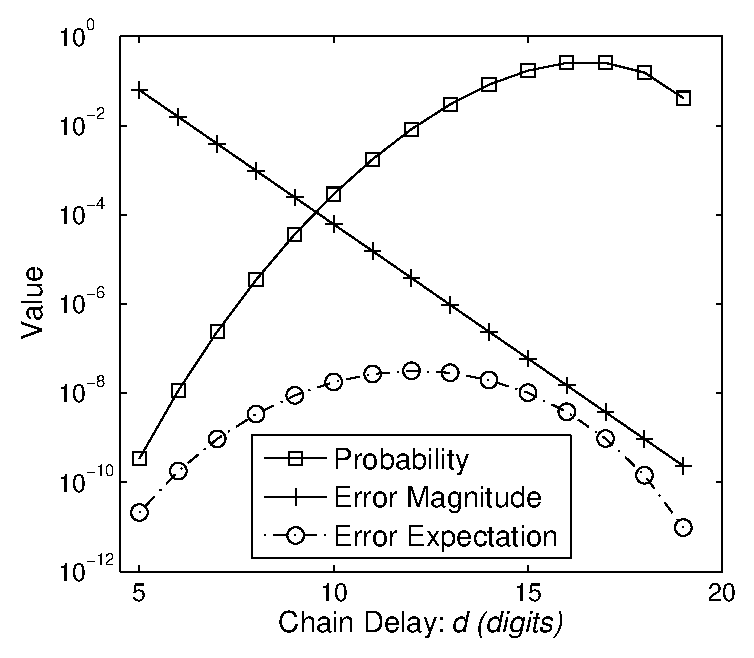
\includegraphics[width=1.7in]{./Figures/PE32.eps}
  \end{minipage}
  }
  \vspace{-3ex}
  \caption{Probabilities of different chain delay, the corresponding magnitude of overclocking error and the combination of both in terms of error expectation in a radix-2 OM.}
  \label{Fig:Probability_Error_Mean}
  \vspace{-2ex}
\end{figure}

\section{Case Study: Image Filter}\label{Sec:CaseStudy}
\subsection{Experimental Setup}
<<<<<<< HEAD
The benefits of the proposed methodology are demonstrated by using a Gaussian image filter with two types of computer arithmetic. One is the radix-2 traditional arithmetic with data represented using 2's complement. In this case, speed-optimized adders and multipliers are created using Xilinx Core Generator \cite{Virtex6}. The other is the radix-2 online arithmetic, with the basic building blocks as described in Section~\ref{OnlineAdderSection} and Section~\ref{OnlineMultSection}. In this case, all inputs and outputs are represented in the online format. In order to achieve the desired latency between input and output, both designs are overclocked and the errors seen at the output are recorded. The results are obtained from a Xilinx Virtex-6 FPGA through post place-and-route simulations. In our experiments, the results are evaluated in terms of mean relative error (MRE), which represents the percentage of error at outputs, as given by (\ref{Eq:MRE}) where $E_{error}$ and $E_{out}$ refer to the mean value of error and correct output, respectively.
=======
The benefits of the proposed methodology are demonstrated by using a $3\times3$ Gaussian image filter with two types of computer arithmetic. One is the radix-2 traditional arithmetic with data represented using 2's complement form. In this case, speed-optimized adders and multipliers are created using Xilinx Core Generator \cite{XilinxMult}. The other is the radix-2 online arithmetic, with the basic building blocks as described in Section~\ref{subsec:OnlineAdder} and Section~\ref{subsec:OnlineMultiplier}. In this case, all inputs and outputs are represented in the online format. In order to achieve the desired latency between input and output, both designs are overclocked and the errors seen at the output are recorded. The results are obtained from a Xilinx Virtex-6 FPGA through post place-and-route simulations. The results are evaluated in terms of mean relative error (MRE), which represents the percentage of error at outputs, as given by (\ref{Eq:MRE}) where $E_{error}$ and $E_{out}$ refer to the mean value of error and correct output, respectively.
>>>>>>> kan
%
\begin{eqnarray}\label{Eq:MRE}
\scriptsize
  MRE=\left|\frac{E_{error}}{E_{out}}\right|\times100\%
  %MRE=\left|{E_{error}}/{E_{out}}\right|\times100\%
\end{eqnarray}
\normalsize
%
%Since the redundant digit set is used in online arithmetic, a signed integer number within $[-2^N,2^N-1]$ can be represented using $N$ digits. However the representation range is $[-(2^{N-1},2^{N-1}-1)]$ with $N$ digits using 2's complement number system. For a valid comparison, an $N$-digit image filter using online arithmetic is employed against an $(N+1)$-digit design using traditional arithmetic.
In our experiments, two types of input data are utilized. One is randomly sampled from a uniform distribution of $N$-digit numbers. This type is referred to as ``Uniform Independent (UI) inputs''. The other is called ``real inputs'', which are the pixel values of several $512\times512$ benchmark images.

\vspace{-1ex}
\subsection{Quantify the Impact of Overclocking}
The values of overclocking error of the image filter based on traditional arithmetic (dotted lines) and online arithmetic (solid lines) when $N=8$ are illustrated in Figure \ref{Fig:MRE_ImageFilter}. According to the timing analysis tool, the rated operating frequencies of the two designs are $168.7$MHz and $148.3$MHz, respectively. However as seen in Figure \ref{Fig:MRE_ImageFilter}, for both input types the online image filter actually operates at a higher frequency without timing violations in comparison to the design using traditional arithmetic. In addition, this error-free frequency is even larger when using the real image data as inputs, since the real data do not exactly follow the uniform distribution or the independent assumption. In Figure \ref{Fig:MRE_ImageFilter} the ``Lena'' benchmark image is used as the real inputs.
%
\begin{figure}
    \centering
    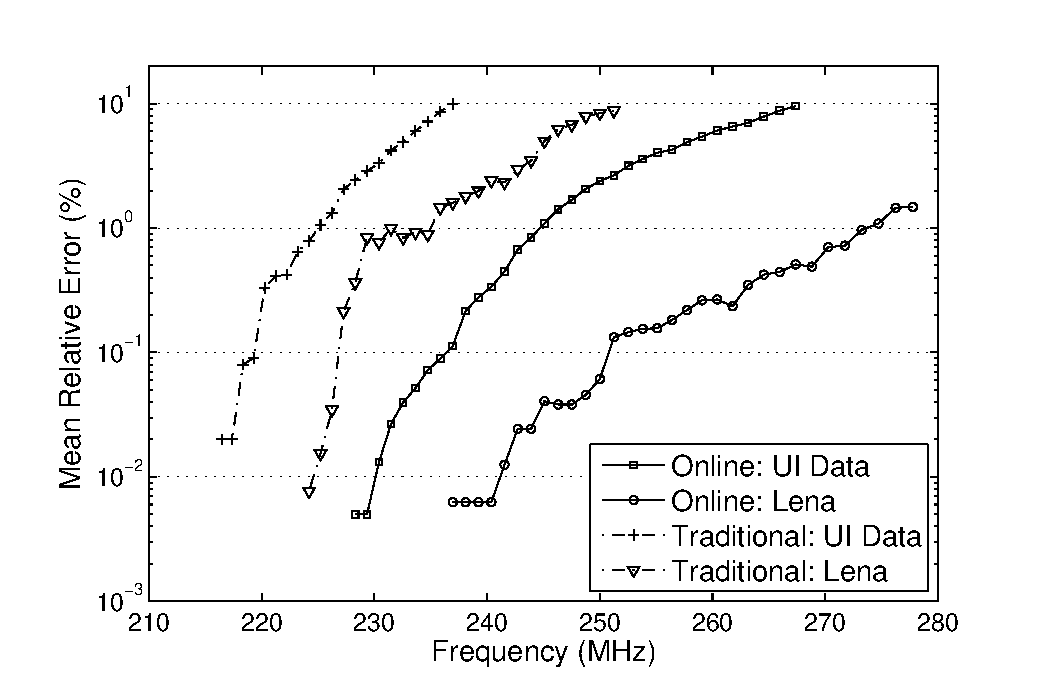
\includegraphics[width=.48\textwidth]{./Figures/MRE.eps}
    \vspace{-4ex}
    \caption{Overclocking error in an image filter with two types of computer arithmetic: online arithmetic and standard binary arithmetic, of which the rated frequencies are 148.3MHz and 168.7MHz, respectively, according to the timing analysis tool.}
    \label{Fig:MRE_ImageFilter}
    \vspace{-2ex}
\end{figure}

%\subsection{Sensitivity of Overclocking Error}
\vspace{-1ex}
If errors can be tolerated, we may allow timing violations to happen for better performance. The sensitivity of overclocking error for a given arithmetic can be evaluated by the data slope in Figure~\ref{Fig:MRE_ImageFilter}. For instance under an error budget of $1\%$~MRE, using the UI inputs the frequency of the traditional design can be improved by $3.89\%$ with respect to the maximum frequency without errors, whereas the design with online arithmetic can be overclocked by $6.85\%$. This indicates that online arithmetic is less sensitive to overclocking, as illustrated in Section \ref{Sec:MeanError}. The difference is even greater using real image data: $13.74\%$ frequency speedup using online arithmetic against $4.04\%$ with traditional arithmetic, because fewer long chains are generated with real inputs.\vspace{-1ex}

The output images for both design scenarios are presented in Figure \ref{Fig:LenaImage}. Since the overclocking errors are in the LSDs of the results with online arithmetic, the degradation on the image can be hardly observed. This leads to ``salt and pepper noise''. In contrast, timing violations cause error in the MSDs with traditional arithmetic.  Meanwhile, errors in the MSDs would result in large noise power and therefore the signal-to-noise ratio (SNR) for the traditional design is small.

\begin{figure}[htb]
  \vspace{-2.5ex}
  \centering
  \subfigure[1.05$f_0$,~SNR=38.3dB]{
  \begin{minipage}[c]{0.24\textwidth}
    \centering
    
\includegraphics[width=1.3in]{./Figures/Lena/Online_T404.eps}
  \end{minipage}%
  }% This is important! use % to indicate same line, otherwise new line
  \subfigure[1.05${f_0}'$,~SNR:21.5dB]{
  \begin{minipage}[c]{0.24\textwidth}
    \centering
    
\includegraphics[width=1.3in]{./Figures/Lena/Trad_T426.eps}
  \end{minipage}
  }\vspace{-1ex}
  \subfigure[1.15$f_0$,~SNR:36.2dB]{
  \begin{minipage}[c]{0.24\textwidth}
    \centering
    
\includegraphics[width=1.3in]{./Figures/Lena/Online_T370.eps}
  \end{minipage}
  }%
  \subfigure[1.15${f_0}'$,~SNR:9.0dB]{
  \begin{minipage}[c]{0.24\textwidth}
    \centering
    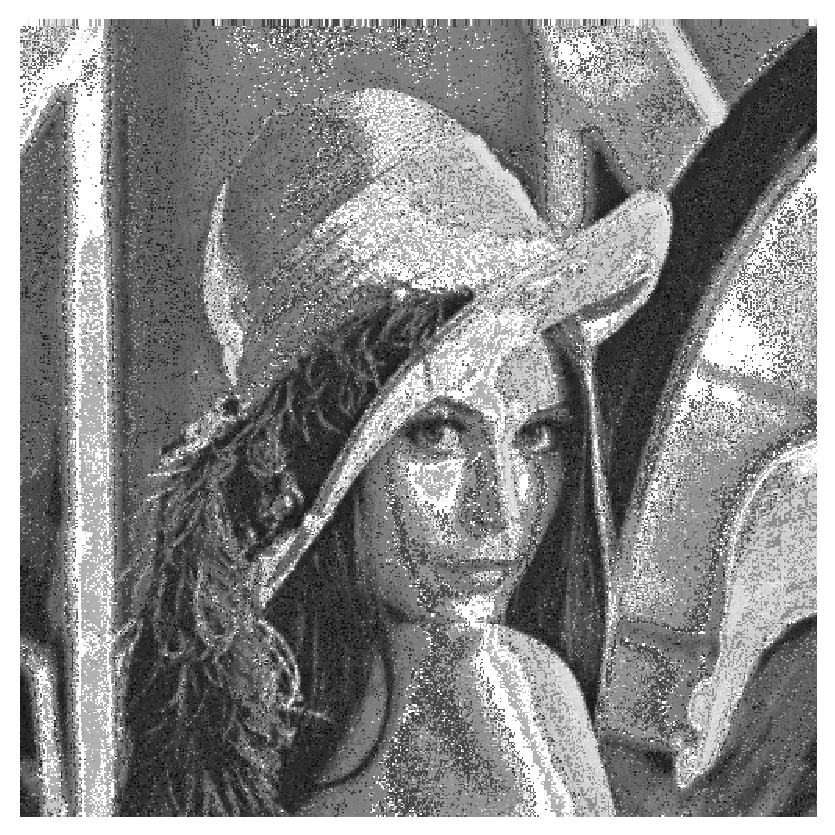
\includegraphics[width=1.3in]{./Figures/Lena/Trad_T390.eps}
  \end{minipage}
  }\vspace{-1ex}
  \subfigure[1.25$f_0$,~SNR:26.7dB]{
  \begin{minipage}[c]{0.24\textwidth}
    \centering
    
\includegraphics[width=1.3in]{./Figures/Lena/Online_T340.eps}
  \end{minipage}%
  }% same line
  \subfigure[1.25${f_0}'$,~SNR:8.5dB]{
  \begin{minipage}[c]{0.24\textwidth}
    \centering
    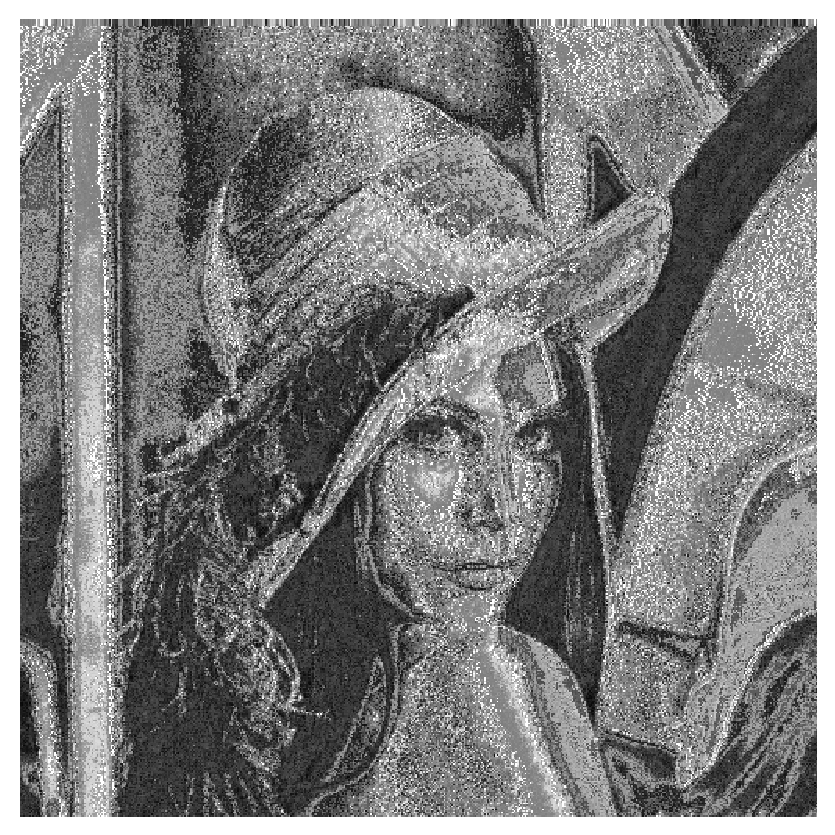
\includegraphics[width=1.3in]{./Figures/Lena/Trad_T358.eps}
  \end{minipage}
  }
\vspace{-2ex}
\caption{Output images of image filter using online arithmetic (left column) and traditional arithmetic (right column), where $f_0$ and ${f_0}'$ denote the maximum error-free frequencies for each design.}
\label{Fig:LenaImage}
\vspace{-1ex}
\end{figure}

<<<<<<< HEAD
\vspace{-1ex}
\subsection{Potential Benefits in Circuit Design}
In general, our results could be of interest to a circuit designers in two ways. By choosing different arithmetic and data representations, either a circuit can be designed to operate at a certain frequency with the minimum possible MRE, or a given error budget specified by the algorithm designer can be met with the fastest achievable frequency. For the first case, the experimental results obtained by UI inputs and 4 benchmark images are summarized in Table~\ref{Tab:MRE_Redu_Freq} in terms of the relative reduction of MRE as given by (\ref{Eq:MRE_Reduction}) where $MRE_{OL}$ and $MRE_{Trad}$ denote the value obtained with online arithmetic and with traditional arithmetic, respectively, and in Table \ref{Tab:SNR_Impro_Freq} for the differences of SNR.
=======
%\vspace{-1ex}
%\subsection{Potential Benefits in Circuit Design}
%In general, our results could be of interest to a circuit designer in two folds. By choosing different arithmetic and data representations, either a circuit can be designed to operate at a certain frequency with the minimum possible MRE, or a given error budget specified by the algorithm designer can be met with the fastest achievable frequency. For the first case,

We also perform experiments using other benchmark images. The results are summarized in Table~\ref{Tab:MRE_Redu_Freq} in terms of the relative reduction of MRE as given by (\ref{Eq:MRE_Reduction}) where $MRE_{OL}$ and $MRE_{Trad}$ denote the value obtained with online arithmetic and with traditional arithmetic, respectively, and in in Table \ref{Tab:SNR_Impro_Freq} for the differences of SNR. In both tables the frequency is normalized to the maximum error-free frequency for each arithmetic. A significant reduction of MRE can be observed using online arithmetic for all input types. The geometric mean reduction varies from $97.3\%$ to $98.2\%$. In addition, larger differences of MRE reduction can be achieved in practice, as long chains occur with even smaller probabilities with real data. Similarly from Table \ref{Tab:SNR_Impro_Freq}, the differences in SNR are $21.4dB\sim43.9dB$.\vspace{1ex}
%
%the experimental results obtained by UI inputs and 4 benchmark images are summarized in Table~\ref{Tab:MRE_Redu_Freq} in terms of the relative reduction of MRE as given by (\ref{Eq:MRE_Reduction}) where $MRE_{OL}$ and $MRE_{Trad}$ denote the value obtained with online arithmetic and with traditional arithmetic, respectively, and .
>>>>>>> kan
%
\begin{eqnarray}\label{Eq:MRE_Reduction}
\scriptsize
  \frac{MRE_{Trad}-MRE_{OL}}{MRE_{Trad}}\times100\%
  %{(MRE_{Trad}-MRE_{OL})}/{MRE_{Trad}}\times100\%
\normalsize
\end{eqnarray}

The area comparison between two designs is illustrated in Table~\ref{Tab:AreaComparison}. While we notice that our approach comes at some increase in area, the FPGA architecture is optimized for conventional arithmetic. For instance, the Virtex series employs dedicated multiplexers and encoders for very fast ripple carry addition~\cite{Virtex6}. Besides, at least 2 orders of magnitude error reduction is obtained for a given frequency in our design, as shown in Figure \ref{Fig:MRE_ImageFilter}. Although the differences in both error and area can be compensated by using more digits with traditional arithmetic, this will result in longer delay and an even larger gap in frequency between two designs.


\begin{table}[tbh]
\vspace{-1ex}
\renewcommand{\arraystretch}{1.1}
\setlength{\tabcolsep}{4.1pt}
\caption{Relative Reduction of MRE with Online Arithmetic for Various Normalized Frequencies.}
\vspace{1ex}
\label{Tab:MRE_Redu_Freq}
\scriptsize
\centering
\begin{tabular}{|c|ccccc|c|}
\hline
\multirow{2}*{\textbf{Inputs}} & \multicolumn{5}{c|}{\textbf{Normalized Frequency}} &
\multirow{2}*{\begin{tabular}{c}\textbf{Geo.}\\\textbf{Mean}\end{tabular}}\\
& 1.05 & 1.10 & 1.15 & 1.20 & 1.25 &\\
\hline
Uniform & 94.5\% & 89.1\% & 90.1\% & 88.3\% & 84.3\% & 89.2\%\\
Lena    & 99.3\% & 99.2\% & 98.9\% & 97.7\% & 94.9\% & 97.9\%\\
Pepper  & 99.7\% & 98.3\% & 98.1\% & 97.2\% & 95.1\% & 97.7\%\\
Sailboat& 99.5\% & 97.9\% & 97.3\% & 96.8\% & 95.1\% & 97.3\%\\
Tiffany & 99.9\% & 97.6\% & 98.4\% & 97.8\% & 97.2\% & 98.2\%\\
\hline
\end{tabular}
%\vspace{-1ex}
\normalsize
\end{table}

\begin{table}[tbh]
%\vspace{-1ex}
\renewcommand{\arraystretch}{1.1}
\setlength{\tabcolsep}{4.1pt}
\caption{Improvement of SNR (dB) with Online Arithmetic for Various Normalized Frequencies.}
\vspace{1ex}
\label{Tab:SNR_Impro_Freq}
%\scriptsize
\small
\centering
\begin{tabular}{|c|ccccc|}
\hline
\multirow{2}*{\textbf{Inputs}} & \multicolumn{5}{c|}{\textbf{Normalized Frequency}} \\
& 1.05 & 1.10 & 1.15 & 1.20 & 1.25\\
\hline
Lena    & 44.6 & 36.3 & 33.2 & 29.1 & 22.9\\
Pepper  & 35.7 & 28.3 & 28.7 & 25.9 & 24.1\\
Sailboat& 33.7 & 27.5 & 26.3 & 25.0 & 21.7\\
Tiffany & 43.9 & 25.9 & 29.5 & 25.6 & 24.5\\
\hline
\end{tabular}
%\vspace{-1ex}
\normalsize
\end{table}

%For the second design perspective, Table \ref{Tab:MRE_Reduc_Error} illustrates the frequency speedups with different input types when specific error budgets can be tolerated. We see that for all input types using online arithmetic still outperforms the traditional design for each MRE budget in terms of operating frequency. Likewise the geometric mean of frequency speed-ups is larger for real image inputs.\vspace{-1ex}

%\begin{table}[htb]
%\vspace{-2ex}
%\renewcommand{\arraystretch}{1.1}
%\setlength{\tabcolsep}{4.1pt}
%\caption{Relative Improvement in Frequency with Online Arithmetic for Various Error Budgets.}
%\label{Tab:MRE_Reduc_Error}
%\scriptsize
%\centering
%\begin{tabular}{|c|cccc|c|}
%\hline
%\multirow{2}*{\textbf{Inputs}} & \multicolumn{4}{c|}{\textbf{Error Budget}} &
%\multirow{2}*{\begin{tabular}{c}\textbf{Geo.}\\\textbf{Mean}\end{tabular}}\\
%& 0.01\% & 0.1\% & 1\% & 10\% &\\
%\hline
%Uniform & N/A & 4.59\%   & 8.78\%  & 12.83\% & 8.03\%\\
%Lena    & 7.96\% & 11.50\%  & 16.39\% & 13.71\% & 11.88\%\\
%Pepper  & 6.22\% & 8.87\%   & 18.68\% & 15.94\% & 11.32\%\\
%Sailboat& 5.71\% & 8.87\%   & 16.93\% & 15.29\% & 10.70\%\\
%Tiffany & 2.35\% & 6.90\%   & 18.58\% & 12.22\% & 7.79\% \\
%\hline
%\end{tabular}
%\label{Tab:}
%\vspace{-2ex}
%\normalsize
%\end{table}

\begin{table}[bht]
\vspace{-1ex}
\caption{Area Comparison between Two Designs.}
\vspace{.5ex}
\small
\centering
\label{Tab:AreaComparison}
\begin{tabular}{|c|cc|c|}
\hline
\multirow{2}*{\textbf{Metric}} & \multicolumn{2}{c|}{\textbf{Arithmetic Type}} &
\multirow{2}*{\textbf{Overhead}}\\
 & Traditional & Online &\\ \hline
 LUTs   & 912 & 1896 & 2.08 \\ \hline
 Slices & 324 & 525 & 1.62 \\ \hline

\end{tabular}
%\vspace{-1ex}
\normalsize
\end{table}

\section{Conclusion}
In this paper, we have studied the probabilistic behavior of key arithmetic primitives with different computer arithmetic when operating beyond the deterministic region. Through the usage of analytical models and empirical FPGA results, we have demonstrated that significant error reduction and performance improvement can be achieved by using the ``overclocking friendly'' online arithmetic.


%ACKNOWLEDGMENTS are optional
%\section{Acknowledgments}
%This section is optional;
%
% The following two commands are all you need in the
% initial runs of your .tex file to
% produce the bibliography for the citations in your paper.
\bibliographystyle{abbrv}
\bibliography{Reference}  % sigproc.bib is the name of the Bibliography in this case
%  and remember to run:
% latex bibtex latex latex
% to resolve all references
%

\end{document}
